\documentclass[12pt]{article}

\usepackage{amssymb,amsmath,amsfonts,bbm,eurosym,geometry,ulem,graphicx,caption,color,setspace,sectsty,comment,footmisc,caption,natbib,pdflscape,subfigure,array,hyperref, booktabs, tabularx}

\usepackage[T1]{fontenc}
\usepackage[utf8]{inputenc}
\usepackage{babel}
\usepackage[font=small,labelfont={bf,sf},tableposition=top]{caption}

\normalem

\onehalfspacing
\newtheorem{theorem}{Theorem}
\newtheorem{corollary}[theorem]{Corollary}
\newtheorem{proposition}{Proposition}
\newenvironment{proof}[1][Proof]{\noindent\textbf{#1.} }{\ \rule{0.5em}{0.5em}}

\newtheorem{hyp}{Hypothesis}
\newtheorem{subhyp}{Hypothesis}[hyp]
\renewcommand{\thesubhyp}{\thehyp\alph{subhyp}}

\DeclareMathOperator\erfc{erfc}

\newcommand{\red}[1]{{\color{red} #1}}
\newcommand{\blue}[1]{{\color{blue} #1}}

\newcolumntype{L}[1]{>{\raggedright\let\newline\\arraybackslash\hspace{0pt}}m{#1}}
\newcolumntype{C}[1]{>{\centering\let\newline\\arraybackslash\hspace{0pt}}m{#1}}
\newcolumntype{R}[1]{>{\raggedleft\let\newline\\arraybackslash\hspace{0pt}}m{#1}}

\geometry{left=1.0in,right=1.0in,top=1.0in,bottom=1.0in}

\begin{document}

\begin{titlepage}
\title{Dynamic Asset Allocation with Options}
\author{Joseph Clark\thanks{joecmail@gmail.com}  and Robert Swan\thanks{r.swan@qic.com} }
\date{\today}
\maketitle
\begin{abstract}
\noindent We derive replicating portfolios for some commonly used dynamic trading rules. In particular, we show that two commonly used dynamic rules can be replicated with static option portfolios. These replicating portfolios are more precise than the corresponding dynamic rules in the sense that the exposure is always correct at each price. For a rule that changes notional exposure linearly with price the error is linear in variance. 


%\vspace{0in}\\
%\noindent\textbf{Keywords:} key1, key2, key3\\
%\vspace{0in}\\
%\noindent\textbf{JEL Codes:} key1, key2, key3\\

\bigskip
\end{abstract}
\setcounter{page}{0}
\thispagestyle{empty}
\end{titlepage}
\pagebreak \newpage




\doublespacing


\section{Introduction} \label{sec:introduction}

A Dynamic Asset Allocation (DAA) rule is a function from price of an asset $S(t)$ and its valuation $S^*$ to a target exposure:

\[DAA(S(t), S^*) \rightarrow \omega(t) \]

The rule typically specifies a positive position if the price is below the valuation $S^*$ and a negative exposure if it is above. There are two ways to implement such a rule:

\begin{enumerate}
\item Adjust a futures exposure to the asset as $S(t)$ or $S^*$ moves
\item Hold a portfolio of options on the asset that generates a delta (option sensitivity the asset) equal to the target DAA weight for any value of $S(t)$
\end{enumerate}

The approaches are identical in the generation of the target DAA exposure at each rebalancing point. Between these points the option portfolio is more correct since the delta matches the rule at each point, even if the price jumps, whereas the futures portfolio is always ``late''. 

%The portfolio of options that matches the DAA rule can be calculated by matching the target exposure to the delta of a strip of options. Holding the options has the effect of changing the exposure dynamically with price in the same manner as a DAA rebalancing trade. 

A typical DAA rule might linearly increase the exposure if the price is below the valuation and decrease if the price is above valuation between some bounds. A replicating option portfolio sells a constant number of options at evenly spaced strikes between a lower bound $S_{lower}$ and upper bound $S_{upper}$. Each put option below the value adds a fixed amount of delta to the total profile so the combination creates a step function (figure \ref{fig:DAARuleLimitedStrikes}). As the interval approaches zero the option delta profile approaches the target.

\begin{figure}[t] 
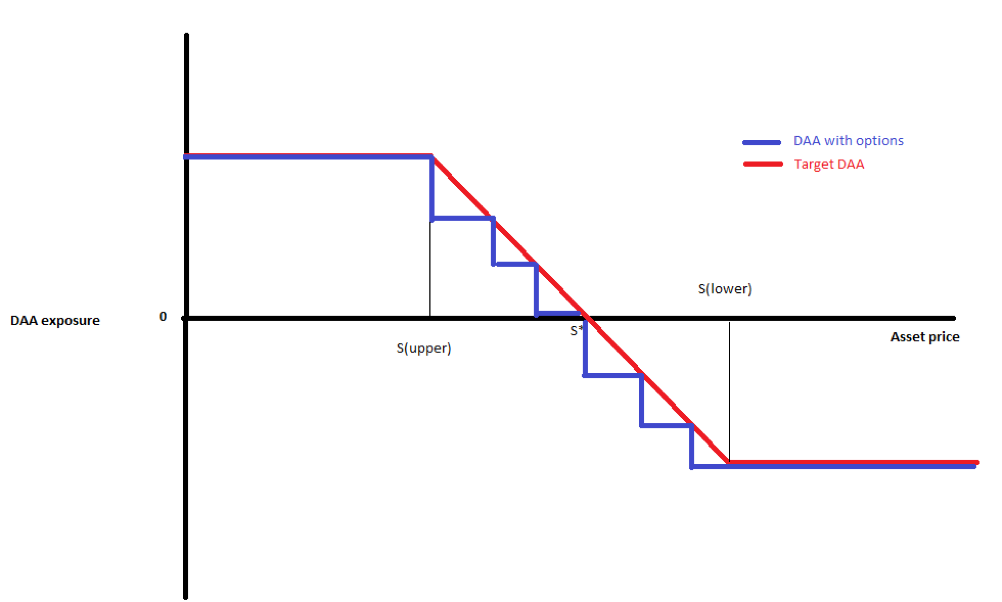
\includegraphics[width=12cm]{figs/DAARuleLimitedStrikes.png}
\centering
\caption{A DAA rule implemented with options}
\label{fig:DAARuleLimitedStrikes}
\end{figure}

This portfolio is linear in delta, but not in notional delta (delta * underlying price). A linear delta notional profile can be generated with a $-dK/K^2$ weights to option strikes $K$. 

This case provides an interesting alternative replication. Option weights of $-dK/K^2$ is part of the replicating portfolio for a log contact, which in turn is part of the replicating portfolio for a variance swap. Certain DAA rules can therefore be seen explicitly as a variance swap plus a rebalanced future.

A more general technique to find the option portfolio to match an arbitrary DAA rule is developed in the appendix. The remainder of the paper demonstrates the machinery more concretely. %The appendix contains technical results concerning spanning a general delta function and the relationship between the weighing function for a strip of options and the portfolio delta.

%In combination, these results construct an option portfolio that provide a pre-defined level of exposure at each possible value. The target DAA rule is a special case of a linear target delta function and can be solved explicitly. 


\section{Preliminaries}

We are interested in portfolio sensitivity (delta) generated by asset allocation rules $\omega(t)$. 

\begin{equation}
 D(\omega(t), S(t)) = \frac{\partial V(\omega(t), S(t))}{\partial S(t)}
\end{equation}
  
Where $V$ is the value of a portfolio given a function $\omega(t)$ specifying weights to replicating assets (for our purposes: futures, options, bonds, log contracts, and variance swaps). 

Delta replicating portfolios are a class of replicating portfolios that produce the same delta: 

\begin{equation*}
R^D(\omega(t)) = \left \{ \omega'(t):   D(\omega'(t), S(t)) =  D(\omega(t), S(t))  \right\}   
\end{equation*}
 

In particular we show how a trading rule that varies with price can be generated with either:

\begin{itemize}
    \item A rebalanced future
    \item A static log contract and future
    \item A static strip of options
    \item A rebalanced future and a static variance swap
\end{itemize}



%\textbf{Replicating portfolio for the log contract}


%\textbf{Replicating portfolio for the variance swap}

%\textbf{Replicating portfolio for linear delta notional}


\section{The relationship between delta and option weights}

The appendix shows that for a weighting function on strikes $\omega(K)$ the delta profile given an expiry price $S(T)$ is 

\begin{equation*}
 D(\omega, S(T)) =  \Omega(S(T)) - \Omega(S^*) 
\end{equation*}

where $\Omega(K) = \int \omega(K)dK$. 

So for constant weights $\bar{\omega}$ the delta is linear in the final price:

\begin{equation*}
 D(\omega, S(T)) =  \Omega(S(T)) - \Omega(S^*) = \bar{\omega} \left( S(T)-S^* \right) 
\end{equation*}

For weights $\bar{\omega}/K^2$ we have

\begin{equation*}
 D(\omega, S(T)) =  \Omega(S(T)) - \Omega(S^*) = \bar{\omega} \left( \frac{1}{S(T)}-\frac{1}{S^*} \right) 
\end{equation*}

For these weights the notional delta (delta * price) is linear in the final price

\begin{equation}
 D(\omega, S(T))S(T) = \bar{\omega} \left( 1-\frac{S(T)}{S^*} \right) \label{eq:NotionalDeltaProfile}
\end{equation}


\section{Spanning with the log contract}

The appendix shows that the log contract paying $\log \frac{S(T)}{S^*}$ has

\[d \log S(t) = \frac{1}{S^*}dS(t) + \int_0^{S^*}d P(K) \frac{-1}{K^2}dK + \int_{S^*}^{\infty}dC(K) \frac{-1}{K^2}dK  \]

The replicating portfolio is: 

\begin{itemize}
    \item $1/S^*$ futures
    \item $-dK/K^2$ puts from 0 to $S^*$ and calls from $S^*$ onward 
\end{itemize}



\section{Spanning with a variance swap}

The linear notional delta option weights ($-dK/K^2$) are the same as for a log contract. The intuition is that a log contract pays the growth rate of the asset, which is the change of value on a constant notional. This means that a DAA rule with a linear notional delta rule can be partly replicated by a variance swap.

The appendix shows that the value of a linear notional delta portfolio can represented as the weighted option payoff or as a function of variance and rebalanced futures

\begin{eqnarray*}
V(S(T), S^*) &=& \int_0^{S^*} P(K) \frac{-1}{K^2}dK + \int_{S^*}^\infty C(K) \frac{-1}{K^2}dK\\
             &=& \int_0^T \frac{dS(t)}{S(t)} -\frac{T}{2}(\sigma^2(t,...) - K^{var})  - \frac{1}{S^*}(S(T)-S^*)
\end{eqnarray*}

Where $K^{var}$ is a variance swap strike and $\sigma^2(t,...) = \frac{1}{T}\int_0^T d \log(S(t))^2$. Differentiating gives the payoff in each period

\begin{eqnarray} \label{varianceReplication}
dV(S(T), S^*) = dS(t)\left(\frac{1}{S(t)} - \frac{1}{S^*}\right)  - 0.5( (d \log(S(t)))^2-K^{var}) 
\end{eqnarray}

This holds approximately in the discrete case

\begin{eqnarray*}
\Delta V(S(T), S^*) \approx \Delta S(t)\left(\frac{1}{S(t)} - \frac{1}{S^*}\right)  - 0.5( (\Delta \log(S(t)))^2-K^{var}) 
\end{eqnarray*}


\section{Example replications}

Suppose we have a DAA rule that targets \$5 notional delta exposure for each 5\% below the valuation and -\$5 for each 5\% below. If the asset is initially at target price $S(0)=S^*=100$ then from (\ref{eq:NotionalDeltaProfile}) we have $\bar{\omega}$ = 100 and there are four possible portfolios that produce the target notional delta:


\textbf{Portfolio 0:}   $100(1/S(t) - 1/S^*)$ futures (rebalanced)

\textbf{Portfolio 1:}  $-100/K^2$  (taking $\Delta K = 1$) put options for $K\leq S^* = 100$ and call options for $K>S^* = 100$ (static)

\textbf{Portfolio 2:}   $100$ log contracts contract and $0.01$ futures (static)

\textbf{Portfolio 3:}   $100 (1/S(t) - 1/S^*)$ futures (rebalanced) and $-50$ variance swap notional  (static)

The portfolio is illustrated for each portfolio across prices between 95 and 105 in tables \ref{tab:port0}-\ref{tab:port3}


   \begin{table}[!ht]
     \caption{Portfolio 0: DAA rebalancing}\label{tab:port0}
     \centering
     \begin{tabularx}{\linewidth}{Xcccccc}\toprule
        \# Contracts across $S(t)$ & 95  & $\ldots$ & 100 & $\ldots$ & 105\\ \midrule
       $S(t)$ & 0.0526 & $\ldots$ & 0& $\ldots$ &  -0.0476   \\
       $\log S(t)$& 0  & $\ldots$ & 0& $\ldots$ &  0   \\
       $\omega(K)$ & 0 & $\ldots$ & 0& $\ldots$ &  0   \\
       Variance &  0 & $\ldots$ & 0& $\ldots$ &  0   \\
       \addlinespace
     \end{tabularx}

   \end{table}

   \begin{table}[!ht]
     \caption{Portfolio 1: Static option replication}\label{tab:port1}
     \centering
     \begin{tabularx}{\linewidth}{Xcccccc}\toprule
         \# Contracts across $S(t)$& 95  & $\ldots$ & 100 & $\ldots$ & 105\\ \midrule
       
       $S(t)$ & 0 & $\ldots$ & 0& $\ldots$ &  0   \\
       $\log S(t)$& 0 & $\ldots$ & 0& $\ldots$ &  0   \\
       $\omega(K)$ & $-100/K^2$ & $\ldots$ & $-100/K^2$& $\ldots$ &  $-100/K^2$    \\
       Variance &  0 & $\ldots$ & 0& $\ldots$ &  0   \\
       \addlinespace
     \end{tabularx}

   \end{table}
   
   
    \begin{table}[!ht]
     \caption{Portfolio 2: Log contract replication}\label{tab:port2}
     \centering
     \begin{tabularx}{\linewidth}{Xcccccc}\toprule
         \# Contracts across $S(t)$& 95  & $\ldots$ & 100 & $\ldots$ & 105\\ \midrule
       
       $S(t)$ & -0.01 & $\ldots$ & -0.01& $\ldots$ &  -0.01   \\
       $\log S(t)$& 100 & $\ldots$ & 100 & $\ldots$ &  100   \\
       $\omega(K)$ & 0 & $\ldots$ & 0 & $\ldots$ &  0   \\
       Variance &  0 & $\ldots$ & 0& $\ldots$ &  0   \\
       \addlinespace
     \end{tabularx}

   \end{table}
   
   
    \begin{table}[!ht]
     \caption{Portfolio 3: Variance swap replication}\label{tab:port3}
     \centering
     \begin{tabularx}{\linewidth}{Xcccccc}\toprule
        \# Contracts across $S(t)$ & 95  & $\ldots$ & 100 & $\ldots$ & 105\\ \midrule
       
       $S(t)$ & 0.0526 & $\ldots$ & 0& $\ldots$ &  -0.0476\\ 
       $\log S(t)$& 0 & $\ldots$ & 0& $\ldots$ &  0   \\
       $\omega(K)$ & 0 & $\ldots$ & 0 & $\ldots$ &  0   \\
       Variance &  50 & $\ldots$ & 50& $\ldots$ &  50   \\
       \addlinespace
     \end{tabularx}

   \end{table}

\section{Discussion}

Asset allocation rules that vary exposure with price are common in the wild. By construction these rules are ``late'' in the sense that the exposure after rebalancing is relevant to the previous price move. Using a portfolio of options solves this problem since by construction the delta adjusts correctly as the price moves. 

This construction is short volatility: intuitively since it sells as the price increases and buys as the price decreases, and explicitly in the replicating portfolio which is short a strip of options. In the special case of a rule targeting linear notional delta changes the portfolio can be made precise by adding a short variance swap.

%If there are no underlying option markets, the price will be determined by market preferences for variance. The replicating portfolio sells a strip of options on the exchange rate $m_p^T$. The delta hedged replicating portfolio payoff is decreasing in the variance of  $m_p^t$. Risk averse investors have decreasing utility in variance and would require a premium to sell these options (see \cite{CarrWu09}). Equally, equity holders in the CPM will equally require compensation via a positive transaction fee for the options embedded in their payoff.   

%It's notable that the replicating portfolio bears a passing resemblance to the $1/K^2$ strikes used to replicate the log contract needed for a variance swaps (see \cite{Derman99}}.





\singlespacing
\setlength\bibsep{0pt}
\bibliographystyle{my-style}
\bibliography{Placeholder}



\clearpage

\onehalfspacing

%\section*{Tables} \label{sec:tab}
%\addcontentsline{toc}{section}{Tables}



%\clearpage

%\section*{Figures} \label{sec:fig}
%\addcontentsline{toc}{section}{Figures}

%\begin{figure}[hp]
%  \centering
%  \includegraphics[width=.6\textwidth]{../fig/placeholder.pdf}
%  \caption{Placeholder}
%  \label{fig:placeholder}
%\end{figure}




\clearpage

\section*{Appendix: Spanning results  } \label{sec:appendixa}

\subsection*{Spanning delta with options}

The delta of a portfolio of puts up to $K^*$ and calls beyond is 

\[  D(\omega, S(t)) = \int_{0}^{K^*} \omega^{put}(K) D(P(K))dK  + \int_{K^*}^\infty \omega^{call}(K) D(C(K))dK \]

Where $D(P)$, $D(C)$ are the delta of the puts and calls. This simplifies to 

\[  D(\omega , S(t)) = \int_{0}^{\infty} \omega(K) D(P(K))dK  + \int_{K^*}^{\infty}\omega(K)dK \]

At expiry this is 

\[  D(\omega , S(T)) = \int_{S}^{\infty} -\omega(K) dK  \int_{K^*}^{\infty}\omega(K)dK \]

Writing $\Omega(K) = \int \omega(K)dK$

\[  D(\omega , S(T)) = \Omega(S(T))-\Omega(K^*)\]

\subsection*{Spanning the log contract}

Any function $W(S(T))$ of the final payoff can be spanned with (see \cite{JarrowGreen87})

\[W(S(T)) = W(A)e^{-rt} + W'(A)(S(T)-Ae^{-rt}) + \int_0^A P(K)W''(K)dK + \int_A^\infty C(K)W''(K)dK\]

For $W(S(T))=\log(S(T))$ and $A=K^*$ and assuming rates are zero this is 

\[ \log(S(T)) = \log(K^*) + \frac{1}{K^*}(S(T)-K^*) + \int_0^{K^*}P(K) \frac{-1}{K^2}dK + \int_{K^*}^{\infty}C(K) \frac{-1}{K^2}dK  \]

Differentiating gives 

\[d \log S(t) = \frac{1}{K^*}dS(t) + \int_0^{K^*}d P(K) \frac{-1}{K^2}dK + \int_{K^*}^{\infty}dC(K) \frac{-1}{K^2}dK  \]

This means the log contract is replicated with
\begin{itemize}
    \item $1/K^*$ futures
    \item $-dK/K^2$ puts from 0 to $K^*$ and calls from $K^*$ onward
\end{itemize}

\section*{Spanning the variance swap}

We use the standard construction for a variance swap (see \cite{Derman99}) with a general price process

\[ \frac{dS(t)}{S(t} = \mu(t,...)dt + \sigma(t,\ldots)dZ(t) \]

It's lemma on $\log S(t)$ gives

\[d \log S(t) = (\mu - 0.5 \sigma^2)dt + \sigma dZ(t) \]

Taking the difference between the orginal process and this is 

\[ \frac{dS(t)}{S(t)} - d\log S(t) = 0.5 \sigma^2 dt \]

Integrating between $0$ and $T$ gives the variance

\[V \equiv \frac{1}{2}\int \sigma^2(t,\ldots) = \frac{2}{T} \left( \int_0^T \frac{dS(t)}{S(t)} -\log \frac{S(T)}{S(0)} \right) \]

This means that a variance contract can be replicated with a rebalanced $\frac{1}{S(t)}$ futures positon and a short log contract.

The discrete version is 

\[ \frac{\Delta S(t)}{S(t)} - \Delta \log S(t) \approx 0.5 (\Delta \log S(t))^2 dt = 0.5 r(t)^2 \]

Where $r(t)$ is the log return.


\begin{thebibliography}{}


\bibitem{CarrWu09} Carr, P., Wu, L., \textit{Variance risk premiums.} Review of Financial Studies 22, 1311–1341, 2009.

\bibitem{Clark14} Clark. J and Swan R.  \textit{Rebalancing with Options} Working Paper, 2014.

\bibitem{Derman99} Emanuel Derman, Kresimir Demeterfi, Michael Kamal, and Joseph Zou. A guide to volatility
and variance swaps. Journal of Derivatives, 6(4):9–32, 1999.

\bibitem{JarrowGreen87} Green R, C., and R.A. Jarrow. \textit{Spanning and completeness in markets with contingent claims.}
Journal of Economic Theory, Vol. 41, No 1, pp. 202-210, 1987.

%\bibitem{Jac2010} Jacobs, Kurt (2010). Stochastic Processes for Physicists. Cambridge University Press. pp. 57–59

%\bibitem{Merton73} Merton, Robert (1973). \textit{Theory of Rational Option Pricing}. Bell Journal of Economics and Management Science. 4 (1): 141–183.


%@article{angeris2019analysis,
%  title={An analysis of Uniswap markets},
%  author={Angeris, Guillermo and Kao, Hsien-Tang and Chiang, Rei and Noyes, %Charlie and Chitra, Tarun},
%  journal={arXiv preprint arXiv:1911.03380},
%  year={2019}


\end{thebibliography}

\end{document}
